\subsection{Data storage \& management}
\subsubsection{Lý thuyết}
\indent Data storage \& management là một phần quan trọng của hệ thống quản trị cơ sở dữ liệu (DBMS). Nó bao gồm các quy trình và công cụ để lưu trữ, quản lý, truy xuất và bảo mật dữ liệu một cách hiệu quả. Các khía cạnh chính của data storage \& management bao gồm:
\begin{itemize}
    \item Lưu trữ dữ liệu: Cách dữ liệu được lưu trữ trên các thiết bị phần cứng như ổ đĩa cứng, SSD, hoặc dịch vụ lưu trữ đám mây.
    \item Quản lý dữ liệu: Các quy trình và công cụ để duy trì tính toàn vẹn, bảo mật và hiệu quả của dữ liệu.
    \item Truy xuất dữ liệu: Cách dữ liệu được truy xuất và trả về cho người dùng hoặc các ứng dụng thông qua các câu truy vấn và các công cụ truy vấn.
    \item Bảo mật dữ liệu: Các biện pháp để bảo vệ dữ liệu khỏi việc truy cập trái phép và tấn công mạng.
\end{itemize}

\subsubsection{Data storage \& management trong PostgreSQL}
\indent PostgreSQL là một hệ quản trị cơ sở dữ liệu quan hệ (RDBMS) và sử dụng mô hình bảng để lưu trữ dữ liệu. Các khía cạnh chính của data storage \& management trong PostgreSQL bao gồm:
\begin{itemize}
    \item Lưu trữ bảng: Dữ liệu được lưu trữ dưới dạng bảng với các cột và hàng có kiểu dữ liệu được xác định trước. 
    \begin{figure}[H]
        \centering
        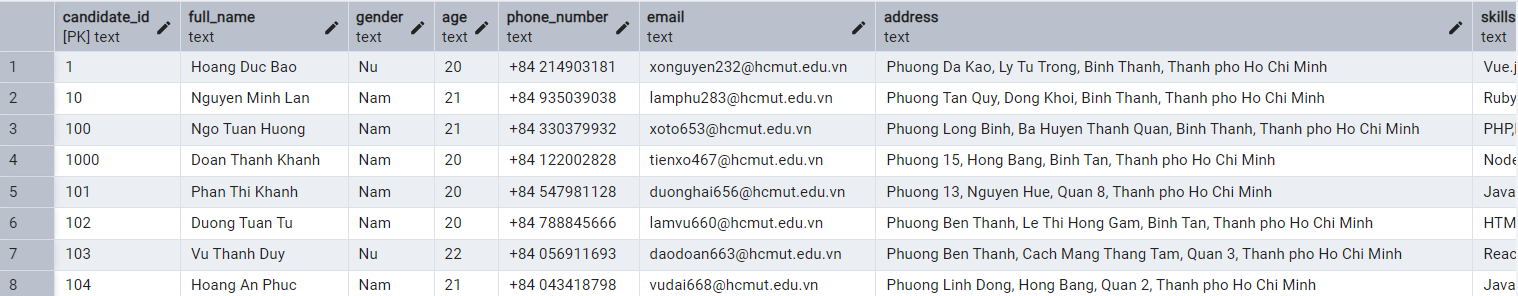
\includegraphics[width=\textwidth]{Image/2.1.2a.png}
        \caption{PostgreSQL lưu trữ dữ liệu dưới dạng bảng}
    \end{figure}
    \item Quản lý không gian lưu trữ: PostgreSQL sử dụng các cơ chế như TOAST (The Oversized-Attribute Storage Technique) để lưu trữ các giá trị lớn ngoài bảng chính.
    \begin{figure}[H]
        \centering
        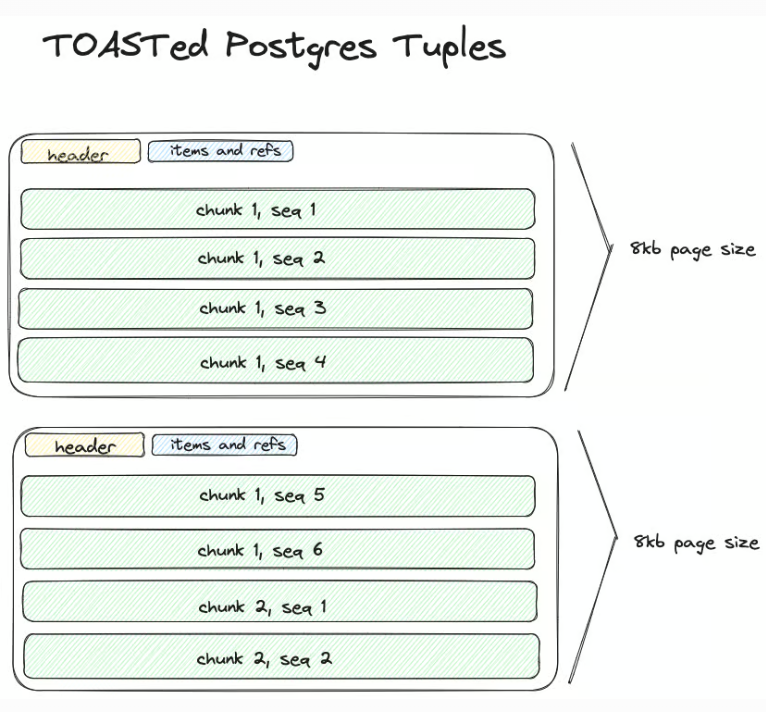
\includegraphics[width=0.9\textwidth]{Image/TOAST.png}
        \caption{Cơ chế TOAST trong PostgreSQL}
    \end{figure}
        \begin{itemize}
            \item Cách TOAST hoạt động
                \begin{itemize}
                    \item Khi một bài viết lớn được chèn vào bảng, PostgreSQL sẽ chia nhỏ nội dung của trường content thành các mảnh nhỏ hơn.
                    \item Các mảnh này được lưu trữ trong một bảng con do TOAST quản lý.
                    \item Bảng chính chỉ lưu trữ các tham chiếu tới các mảnh dữ liệu này.
                \end{itemize}
        \end{itemize}
    \item Truy vấn và tối ưu hóa: PostgreSQL cung cấp các công cụ tối ưu hóa truy vấn để đảm bảo hiệu suất cao khi truy xuất dữ liệu.
    \item Bảo mật và tính toàn vẹn: PostgreSQL hỗ trợ các chức năng bảo mật như kiểm soát quyền truy cập, mã hóa dữ liệu và kiểm tra tính toàn vẹn của dữ liệu.
\end{itemize}

\subsubsection{Data storage \& management trong MongoDB}
\indent MongoDB là một hệ quản trị cơ sở dữ liệu NoSQL và sử dụng mô hình tài liệu để lưu trữ dữ liệu. Các khía cạnh chính của data storage \& management trong MongoDB bao gồm:
\begin{itemize}
    \item Lưu trữ tài liệu: Dữ liệu được lưu trữ dưới dạng tài liệu JSON, cho phép lưu trữ dữ liệu không cấu trúc hoặc một phần cấu trúc. 
    \begin{figure}[H]
        \centering
        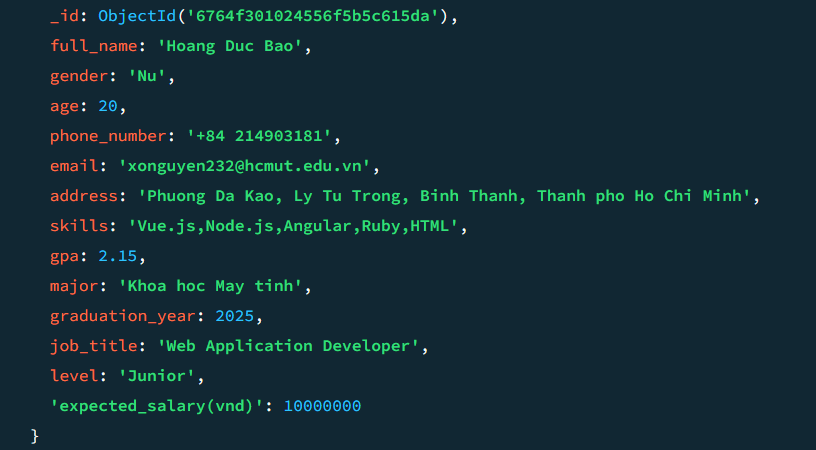
\includegraphics[width=0.9\textwidth]{Image/2.1.3a.png}
        \caption{Mongodb lưu trữ dữ liệu dưới tài liệu}
    \end{figure}
    \item Quản lý không gian lưu trữ: MongoDB sử dụng các cơ chế như sharding để phân chia dữ liệu lên nhiều máy chủ, giúp tăng khả năng mở rộng và hiệu suất.
    \begin{figure}[H]
        \centering
        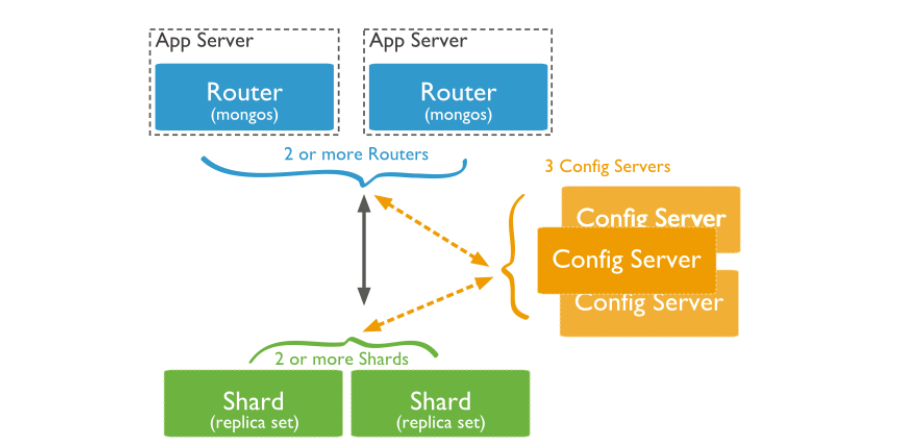
\includegraphics[width=0.9\textwidth]{Image/Sharding.png}
        \caption{Sharding trong MongoDB sử dụng Sharded Cluster}
    \end{figure}
    \item Truy vấn và tối ưu hóa: MongoDB cung cấp các công cụ truy vấn và tối ưu hóa để đảm bảo hiệu suất cao khi truy xuất dữ liệu.
    \item Bảo mật và tính toàn vẹn: MongoDB hỗ trợ các chức năng bảo mật như kiểm soát quyền truy cập, mã hóa dữ liệu và kiểm tra tính toàn vẹn của dữ liệu.
\end{itemize}

\subsubsection{So sánh và kết luận}
\begin{itemize}
    \item Mô hình dữ liệu: PostgreSQL sử dụng mô hình bảng quan hệ, trong khi MongoDB sử dụng mô hình tài liệu JSON.
    \item Hiệu suất: PostgreSQL thường có hiệu suất tốt hơn cho các truy vấn phức tạp và các ứng dụng quan hệ, trong khi MongoDB có hiệu suất tốt hơn cho các ứng dụng với dữ liệu không cấu trúc hoặc một phần cấu trúc.
    \item Khả năng mở rộng: PostgreSQL hỗ trợ mở rộng qua các cơ chế như sharding và replication, nhưng MongoDB được thiết kế từ đầu để mở rộng theo mô hình scale-out.
    \item Tính linh hoạt: MongoDB cung cấp tính linh hoạt cao hơn cho các dữ liệu không cấu trúc, trong khi PostgreSQL cung cấp tính toàn vẹn và tính nhất quán cao hơn cho dữ liệu cấu trúc.
\end{itemize}

\begin{table}[H]
    \centering
    \begin{tabular}{|L{3.2cm}|L{5cm}|L{5cm}|} \hline 
         \textbf{Tiêu chí so sánh }&  \textbf{PostgreSQL}&  \textbf{MongoDB}\\ \hline 
         Mô hình dữ liệu &  Sử dụng các bảng quan hệ. & Sử dụng mô hình tài liệu JSON.\\ \hline 
         Hiệu suất &  Thích hợp cho các truy vấn phức tạp và ứng dụng quan hệ. & Hiệu suất tốt hơn cho dữ liệu phi cấu trúc và bán cấu trúc.\\ \hline 
         Khả năng mở rộng &  Hỗ trợ mở rộng qua cơ chế sharding và replication. &  Mở rộng theo mô hình scale-out.\\ \hline
         Tính linh hoạt &  Cung cấp tính toàn vẹn và tính nhất quán cho dữ liệu cấu trúc. &  Cung cấp tính linh hoạt cao hơn cho các dữ liệu không cấu trúc,.\\ \hline 
    \end{tabular}
    \caption{So sánh về Data storage \& management giữa PostgreSQL và MongoDB}
    \label{tab:data_storage&management}
\end{table}

\textbf{Kết luận:} 
\newpage